% 使用 BHCexam 文档类,并传递选项
\documentclass[windows,list,answers]{BHCexam}
\usepackage{wrapfig}
\begin{document}
\everymath{\displaystyle}
\title{3.1 练习题}

\maketitle

\begin{questions}
    %Questions goes here.
    \question
    试证明确界的唯一性.
    \begin{solution}{1cm}
        \methodonly
        反证.不妨设有$a>b$都为$A$上确界,

        取$0<\varepsilon<a-b$,则由确界定义知$\exists\, a_n>a-\varepsilon>b$且
        $a_n<a$;这与$b$也为上确界矛盾,故上确界唯一.下确界同理可证.
    \end{solution}

    \question
    设对每个$x\in A$成立$x<a$.问:在$\sup A<a$和$\sup A\leqslant a$中哪个是对的?
    \begin{solution}{1cm}
        \methodonly
        后者.显然$\sup A\leqslant a$必然成立.

        设$A=\left\{1-(\frac{1}{2})^n\,\bigg\lvert\,n\in N_+\right\}$,
        显然$x<1$对$x\in A$都成立,而无论多小的$\varepsilon$,都$\exists
            \,n\in N_+\,s.t.\,1-(\frac{1}{2})^n>1-\varepsilon$,即$\sup A=1$.
    \end{solution}
    \question
    设数集$A$以$\beta$为上界,又有数列$\{x_n\}\subset A$和$\lim_{n\to\infty}x_n=\beta.$证明$\beta=\sup A$.
    \begin{solution}{1cm}
        \methodonly
        由收敛定义可知无论多小的$\varepsilon>0$都$\exists\,N\in N_+
            \,s.t.\,n>N,\beta-x_n<\varepsilon\Rightarrow\beta-\varepsilon<x_n$.
        这就是上确界定义.
    \end{solution}
    \question
    求下列数集的上确界和下确界:
    \begin{subquestions}
        \subquestion
        $\{x\in Q\,\lvert\, x>0\};$
        \begin{solution}{1cm}
            \methodonly
            显然下确界是0,上确界是$+\infty$.
        \end{solution}

        \subquestion
        $\{y\,\lvert\, y=x^2,x\in(-\frac{1}{2},1)\};$
        \begin{solution}{1cm}
            \methodonly
            \begin{minipage}{\linewidth}
                \begin{wrapfigure}{r}{3.5cm}
                    \vspace{-2.5cm}
                    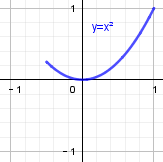
\includegraphics[width=3.5cm]{图一.png}
                    \caption{}
                \end{wrapfigure}
                如右图所示,
                下确界为0,上确界为1.
            \end{minipage}

        \end{solution}

        \subquestion
        $\left\{\left(1+\frac{1}{n}\right)^n \,\bigg\lvert\, n\in N_+\right\};$
        \begin{solution}{1cm}
            \methodonly
            下确界为2,上确界为$e$.

            前已证$\left(1+\frac{1}{n}\right)^n$单调递增且极限为$e$.
        \end{solution}

        \subquestion
        $\{ne^{-n}\,\lvert\, n\in N_+\};$
        \begin{solution}{1cm}
            \methodonly
            前后两项的比值为$\frac{1}{e}\cdot\frac{n+1}{n}<\frac{2}{e}<1$,故数列
            $\left\{\frac{n}{e^n}\right\}$单调递减.而且上一章已证$\left\{\frac{n^q}{p^n}\right\}\to 0(p>1)$,
            所以下确界为0,上确界为$\frac{1}{e}$.
        \end{solution}

        \subquestion
        $\{\arctan x \,\lvert\, x\in (-\infty,+\infty)\};$
        \begin{solution}{1cm}
            \methodonly
            上下确界为$\pm \frac{\pi}{2}$.下证上确界.

            由于$\arctan x$值域在$\left(-\frac{\pi}{2},\frac{\pi}{2}\right)$,而$\tan x$
            在此集合上单调增,故对任意小的$\varepsilon$,欲使$\arctan n>\frac{\pi}{2}-\varepsilon$,
            只需$\tan(\arctan n)=n>\tan\left(\frac{\pi}{2}-\varepsilon\right)$即可.

        \end{solution}

        \subquestion
        $\left\{(-1)^n+\frac{1}{n}(-1)^{n+1}\,\biggl\lvert\, n\in N_+\right\};$
        \begin{solution}{1cm}
            \methodonly
            上下确界为$\pm 1$.

            从感性可以认知到集合中的数从中间向外边(-1和1)扩,对于任意小的$\varepsilon$,只需取
            $n$使$\frac{1}{n}<\varepsilon$即可.
        \end{solution}

        \subquestion
        $\left\{1+n\sin\frac{n\pi}{2}\,\bigg\lvert\, n\in N_+\right\}$.
        \begin{solution}{1cm}
            \methodonly
            上下确界为$\pm \infty$.

            无论多大的M,都存在$n>M$且为$4k+1$(k为正整数)使$1+n\sin\frac{n\pi}{2}=1+n>M$;

            同理也存在$n>-M-10$且为$4k+3$(k为正整数)使$1+n\sin\frac{n\pi}{2}=1-n<M$.
        \end{solution}
    \end{subquestions}

    \question
    证明:
    \begin{subquestions}
        \subquestion
        $\sup\{x_n+y_n\}\leqslant \sup\{x_n\}+\sup\{y_n\}$;
        \begin{solution}{1cm}
            \methodonly
            因为对$n\in N_+$都成立$x_n+y_n<\sup\{x_n\}+\sup\{y_n\}$,故$\sup\{x_n\}+\sup\{y_n\}$
            也为$\{x_n+y_n\}$上界,而由上确界定义(上确界是所有上界中最小的一个)知命题成立.
        \end{solution}

        \subquestion
        $\inf\{x_n+y_n\}\geqslant\inf\{x_n\}+\inf\{y_n\}$.
        \begin{solution}{1cm}
            \methodonly
            解法与上题类似
        \end{solution}
    \end{subquestions}

    \question
    设有两个数集$A$和$B$,且对数集$A$中的任何一个数$x$和数集$B$中的任何一个数$y$成立不等式$x\leqslant y$.
    证明:\,$\sup\{x_n\}\leqslant\{y_n\}$.
    \begin{solution}{1cm}
        \methodonly
        由题知,$\{y_n\}$中元素全是$\{x_n\}$上界,而由定义知命题成立.
    \end{solution}

    \question
    设数集$A$有上界,数集$B=\{x+c\,\lvert\, x\in A\}$,其中$c$是一个常数.证明:\,
    \[\sup B=\sup A+c,\inf B=\inf A+c.
    \]

    \begin{solution}{1cm}
        \methodonly
        只证上确界.

        显然$\sup B\leqslant\sup A+c$.
        由定义知无论多小的$\varepsilon$,都存在$n$使得$a_n>\sup A-\varepsilon$,
        即$a_n+c>\sup A+c-\varepsilon$,故$\sup B=\sup A+c$.下确界证法完全类似.
    \end{solution}

    \question
    设$A,B$是两个有上界的数集,又有数集$C\subset \{x+y\,\lvert\, x\in A,y\in B\}$,则
    $\sup C\leqslant \sup A+\sup B$.举出成立严格不等号的例子.
    \begin{solution}{1cm}
        \methodonly
        挺显然的.

        因为由定义有$x<\sup A,y<\sup B$,即$\sup A+\sup B$是$\{x+y\,\lvert\,x\in A,y\in B\}$
        一个上界,
        
        故有$\sup \{x+y\,\lvert\,x\in A,y\in B\}\leqslant\sup A+\sup B$,而
        $C\subset \{x+y\,\lvert\,x\in A,y\in B\}$,
        
        所以$\sup C\leqslant \{x+y\,\lvert\,x\in A,y\in B\}\leqslant\sup A+\sup B$.

        例如$A=\{1,2\},B=\{2,3\};C=\{3\}$.
    \end{solution}

    \question
    设$A,B$是两个有上界的数集,又有数集$C\supset  \{x+y\,\lvert\, x\in A,y\in B\}$,则
    $\sup C\geqslant \sup A+\sup B$.举出成立严格不等号的例子.
    \begin{solution}{1cm}
        \methodonly
        与上题完全类似.
    \end{solution}
    (合并以上两题可见:当且仅当$C=\{x+y\,\lvert\, x\in A,y\in B\}$时成立$\sup C=\sup A+\sup B$.)

\end{questions}

\end{document}